\documentclass[letterpaper,12pt]{article}
\usepackage[utf8]{inputenc}
\usepackage{xcolor}
\usepackage{todonotes}

\newcommand{\page}[1]{\subsubsection*{\textbf{\underline{Page #1 of 4}}:}}

\usepackage{xparse}
\usepackage{xcolor}
\usepackage[]{graphicx}
\usepackage{mdframed}
\usepackage{geometry}
\usepackage{siunitx}
\usepackage{calc}

\NewDocumentCommand{\revised}{om}{{\leavevmode\color{blue}#2}}
\NewDocumentCommand{\reviewitem}{m}{\fcolorbox{blue}{yellow}{\color{blue}#1}}
\NewDocumentCommand{\location}{m}{(#1)}

\mdfsetup{skipabove=\topskip}
\mdfdefinestyle{theoremstyle}{%
linecolor=gray!50,
linewidth=1pt,%
frametitlerule=true,% 
frametitlebackgroundcolor=gray!20,
% innertopmargin=\topskip,
}
\mdtheorem[style=theoremstyle]{numcomment}{Comment}
\NewDocumentEnvironment{comment}{o}
  {\IfNoValueF{#1}{\setcounter{numcomment}{#1-1}}\numcomment}
  {\endnumcomment}
\NewDocumentEnvironment{revisedto}{}{\color{blue}\em}{}
 
\begin{document}

\begin{frame}[t]
  % Huge text after this
  \huge{Paper Reading of \texttt{Path Confidence based Lookahead Prefetching @MICRO2016}\cite{kim2016path}}

  \bigskip
\end{frame}

\section{Summary}
Prior than this work, the naive implementation is next-line or stride prefetcher, which only has ability of offset prefetcher with fixed distance. Inria proposed Bast Offset prefether \cite{michaud2016best} on HPCA 2016. which has varied offset through a learning procedure and maintain a RR table to record the completed prefetch requres.\\
\begin{center}
  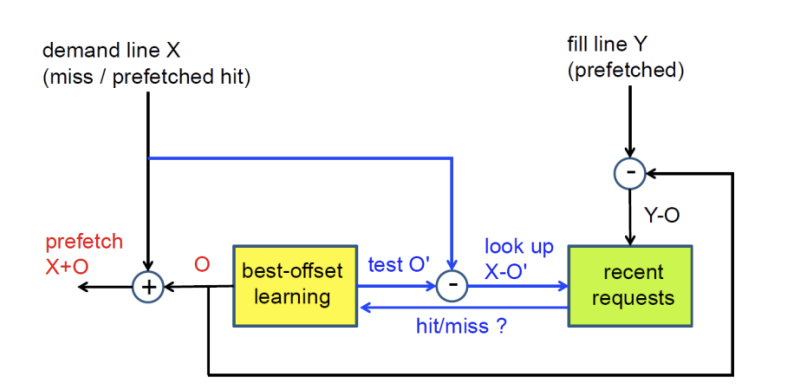
\includegraphics[width=\textwidth]{RRtable.png}
\end{center}
\begin{enumerate}
  \item Prefetch Y, save the current offset O=>Y-O to the RR table
  \item In learning phase, all the offsets in list will be tested,
        \begin{enumerate}
          \item If hit in RR table, score + 1
          \item If learning phase finish or some offset reach SCORE\_MAX, the phase ends.
          \item The offset with highest score will be the best offset. New learning phase starts.
        \end{enumerate}
\end{enumerate}
Taking from Best-Offset Prefetcher, we know this is a one-degree prefetcher, it will turn off the prefetcher if the best score is too low, MSHR threshold varied depends on best offset score and L3 access rate.

SPP frist uses a compressed history based scheme that accrately predicts complex address patterns, then records the complex patterns accross physical pag boundaries and continues prefetching as soon as they move to new pages, the prediction is based on the confidence which is a metrics adaptively throttle itself on a pre-prefetch stream basis.

\begin{figure}[h]
  \centering
  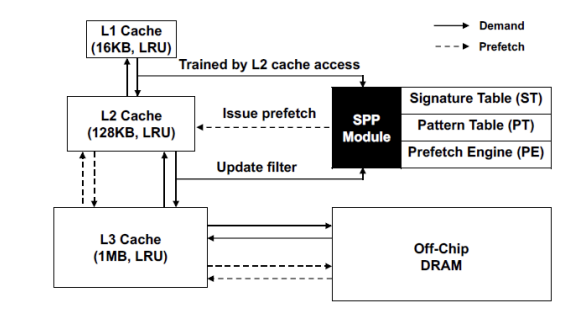
\includegraphics[width=0.5\textwidth]{spp.png}
  $\qquad \qquad$
  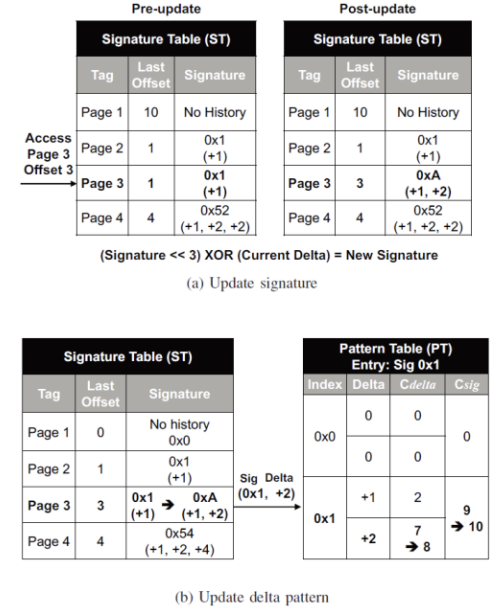
\includegraphics[width=0.3\textwidth]{pattern.png}
\end{figure}
The Signature based table updating amid L2 acess a page, the table will update with offset, offset delta used to generate new signature, and the prior speculative signature deltas is used to modifying pattern table. The same pattern will have the same signature to reduce the storage of PT store entries.
\begin{center}
  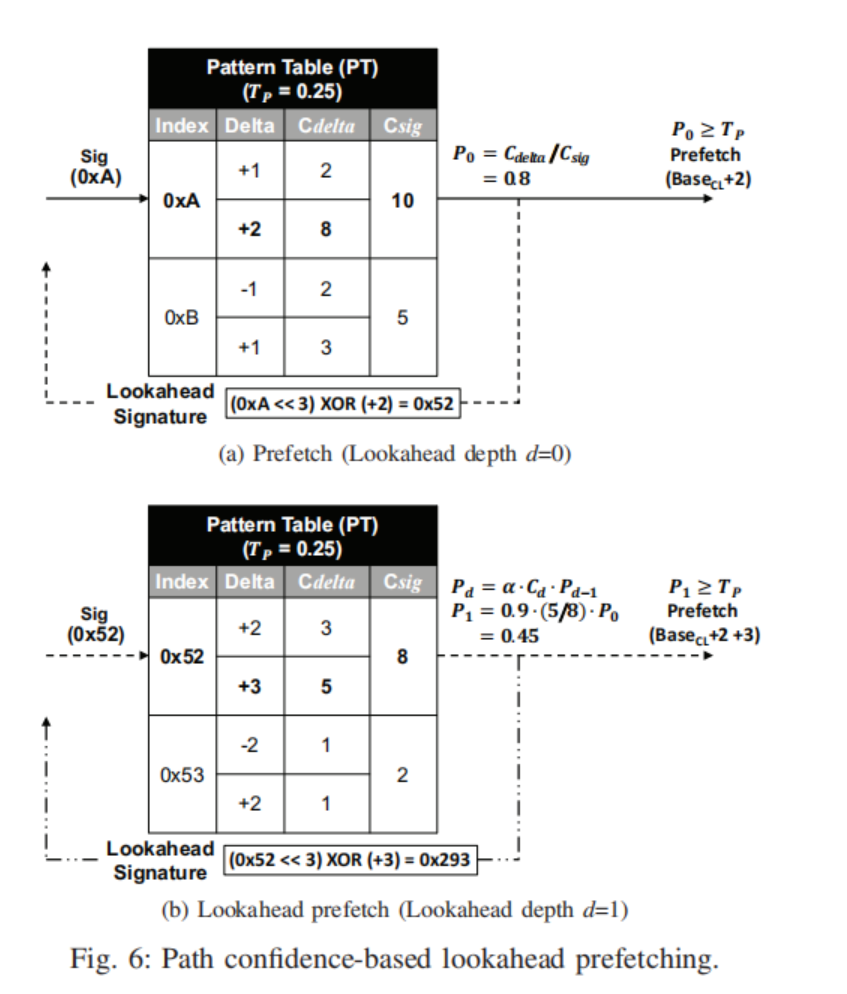
\includegraphics[width=\textwidth]{lookahead.png}
\end{center}
The prefetching processes is listed following:
\begin{enumerate}
  \item Search the signature of
        current accessed page
  \item Choose the delta with highest
        probability $P_i
          (C_{delta}/C_{sig})$ of $i_{th}$
        prefetch depth
  \item If multiply of all P larger than
        threshold
        \begin{enumerate}
          \item Prefetch current address +
                delta
          \item Use delta to update signature
                and access pattern table
                again
        \end{enumerate}
  \item If P < threshold, the procedure end
\end{enumerate}
\section{Strengths}
 The SPP prefetcher can learn the semantic of page fetching accross the page bound accurately that can break the "Memory Wall", which is the gap between processor and memory.

\section{Weaknesses}
 The possible be leveraged by side channel attacks.
\section{How to improve}
The perceptron-based prefetch filtering\cite{10.1145} has a lot variant to the current design of the SPP prefetcher, for instance, perceptron learning for microarchitectural prediction was introduced for branch prediction. PPF enables the underlying prefetcher to be tuned more aggressively, increasing coverage by filtering out the increasing number of faulty prefetches that such aggressive tuning implies. We also investigate several aspects for training the PPF's perceptron layer to recognize false prefetches. PPF outperforms the underlying prefetcher alone on a memory-intensive subset of the SPEC CPU 2017 benchmarks by 11.4\% for a 4-core setup and 3.78\% for a single-core configuration.
\section{Related Work}
\begin{enumerate}
  \item Page aware prefetcher \cite{vavouliotis2022page} at page level, which augments the MSHR to implement PPM. See both need a better prefetcher that knows the semantic of page size(permission/size). Such things spatial prefetcher, the previous 4KB physical page boundary is limited by non-contiguous physical memory, large page prefetch also has side channel problems. Their implementation is a TLB plus an address translator. translator and cache size are passed into MSHR, and the prefetcher still uses the old Signature Path Prefetcher (a prefetcher that uses throttling confidence threshold, is a part of DMP (data memory-dependent prefetcher)).
  \item The Cletcher team attacked the similar prefetecher design on M1 \cite{augury}, they categorized them as data memory-dependent prefetcher which is a wider range of SPP prefetcher. They found inside the M1 L3 that can do address-correlated work to metigate the pointer chasing. They leverage the timing difference of the prefetcher prediction and compose array of pointer to leverage the timing the difference.
\end{enumerate}
\bibliographystyle{ACM-Reference-Format}
\bibliography{paper01}

\end{document}

